\documentclass{beamer}
\usepackage[utf8]{inputenc}

\usetheme{Madrid}
\usecolortheme{default}
\usepackage{amsmath,amssymb,amsfonts,amsthm}
\usepackage{txfonts}
\usepackage{tkz-euclide}
\usepackage{listings}
\usepackage{adjustbox}
\usepackage{array}
\usepackage{tabularx}
\usepackage{gvv}
\usepackage{lmodern}
\usepackage{circuitikz}
\usepackage{tikz}
\usepackage{graphicx}

\setbeamertemplate{page number in head/foot}[totalframenumber]

\usepackage{tcolorbox}
\tcbuselibrary{minted,breakable,xparse,skins}



\definecolor{bg}{gray}{0.95}
\DeclareTCBListing{mintedbox}{O{}m!O{}}{%
  breakable=true,
  listing engine=minted,
  listing only,
  minted language=#2,
  minted style=default,
  minted options={%
    linenos,
    gobble=0,
    breaklines=true,
    breakafter=,,
    fontsize=\small,
    numbersep=8pt,
    #1},
  boxsep=0pt,
  left skip=0pt,
  right skip=0pt,
  left=25pt,
  right=0pt,
  top=3pt,
  bottom=3pt,
  arc=5pt,
  leftrule=0pt,
  rightrule=0pt,
  bottomrule=2pt,
  toprule=2pt,
  colback=bg,
  colframe=orange!70,
  enhanced,
  overlay={%
    \begin{tcbclipinterior}
    \fill[orange!20!white] (frame.south west) rectangle ([xshift=20pt]frame.north west);
    \end{tcbclipinterior}},
  #3,
}
\lstset{
    language=C,
    basicstyle=\ttfamily\small,
    keywordstyle=\color{blue},
    stringstyle=\color{orange},
    commentstyle=\color{green!60!black},
    numbers=left,
    numberstyle=\tiny\color{gray},
    breaklines=true,
    showstringspaces=false,
}
%------------------------------------------------------------
%This block of code defines the information to appear in the
%Title page
\title %optional
{9-9.6-17}
\date{January 9, 2025}
%\subtitle{A short story}

\author % (optional)
{Harshil Rathan Y - EE24BTECH11064}



\begin{document}


\frame{\titlepage}
\begin{frame}{Question}
Find the equation of a curve passing through the point (0, 2) given that the sum of the coordinates of any point on the curve exceeds the magnitude of the slope of the tangent to the curve at that point by 5
\end{frame}
\begin{frame}{allowframebreaks}
\frametitle{Equation}

    \centering
    
    \label{tab:parameters}
    \begin{align}
         x+y = \frac{dy}{dx} + 5
    \end{align}
    \begin{align}
        \frac{dy}{dx} - y= x-5
    \label{0.2}
    \end{align}
   
\end{frame}


\begin{frame}{Theoretical Solution}
Comparing \ref{0.2} with $\frac{dy}{dx} + Py = Q$, 
  \begin{align}
      P=-1 \text{ and } Q = x-5
  \end{align}
I.F is \ref{0.4}
  \begin{align}
       e^{\int P dx} = e^ {-x}
    \label{0.4}
  \end{align}
Solution is \ref{0.5}
\begin{align}
    y \cdot e^{-x} = \int \brak{x-5} e^{-x} \text{ }dx +c 
    \label{0.5}
\end{align}
On applying product rule
\begin{align}
    \int A\cdot B \text{ }dx = A \int B \text{ }dx - \int \frac{d}{dx}(A)\brak{\int B \text{ }dx}dx
\end{align}
\end{frame}
\begin{frame}{allowframebreaks}
\frametitle{Theoretical Solution}
\begin{align}
    y e^{-x} = - (x-5)e^{-x} + \int e^{-x}  dx + c
\end{align}
On Simplyfying 
\begin{align}
     x+y = 4 + c e^x
    \label{0.12}
\end{align}
To find c, put x=0 and y=2 in \ref{0.12}
\begin{align}
     c = -2
\end{align}
The curve equation is 
\begin{align}
    x+y = 4 -2e^x
\end{align}
\end{frame}
\begin{frame}
\frametitle{Solution by Laplace Transform}
\begin{align}
    \frac{dy}{dx} = x+y-5
\end{align}
Applying the Laplace transform to both sides:

\begin{align}
    \mathcal{L}\left\{\frac{dy}{dx}\right\} = \mathcal{L}\left\{x + (y - 5)\right\}
\end{align}
\begin{align}
    sY(s) - y(0) = \frac{1}{s^2} + Y(s) - \frac{5}{s}
\end{align}
\begin{align}
    Y(s) = \frac{\frac{1}{s^2} - \frac{5}{s} + y(0)}{s - 1}
\end{align}
\begin{align}
    Y(s) = \frac{1}{s^2 (s - 1)} - \frac{1}{s (s - 1)} \cdot 5 + \frac{y(0)}{s - 1}
\end{align}
\end{frame}
\begin{frame}
\frametitle{Solution by Laplace Transform}
Inverse Laplace Transform of Each Term
\begin{align}
    \frac{1}{s^2 (s - 1)} = \frac{A}{s} + \frac{B}{s^2} + \frac{C}{s - 1}
\end{align}
\begin{align}
    1 = A\text{ } s\text{ } (s - 1) + B \text{ }(s - 1) + C \text{ }s^2
\end{align}
we get
\begin{align}
    \frac{1}{s^2 (s - 1)} = -\frac{1}{s} -\frac{1}{s^2} + \frac{1}{s - 1}
\end{align}
Taking the inverse Laplace transform
\begin{align}
    \mathcal{L}^{-1}\left\{ \frac{1}{s} - \frac{1}{s - 1} \right\} = -1 - x + e^x
\end{align}
\end{frame}
\begin{frame}
\frametitle{Solution by Laplace Transform}
Inverse Laplace of \( \frac{5}{s (s - 1)} \)
\begin{align}
    \frac{5}{s (s - 1)} = \frac{A}{s} + \frac{B}{s - 1}
\end{align}
\begin{align}
    5 = A (s - 1) + B s
\end{align}
Solving gives \( A = 5 \) and \( B = -5 \)
\begin{align}
    \frac{5}{s (s - 1)} = \frac{5}{s} - \frac{5}{s - 1}
\end{align}
Taking the inverse Laplace transform
\begin{align}
    \mathcal{L}^{-1}\left\{ \frac{5}{s} - \frac{5}{s - 1} \right\} = 5 - 5 e^x
\end{align}

\end{frame}
\begin{frame}{Solution by Laplace Transform}
Inverse Laplace of \( \frac{y(0)}{s - 1} \)
\begin{align}
    \mathcal{L}^{-1}\left\{ \frac{y(0)}{s - 1} \right\} = y(0) e^x
\end{align}
combining the results from all parts, we have the solution for $y(x)$
The general solution too this differential equation is 
\begin{align}
    y(x) = 4 - x + (y(0) - 4) e^x 
\end{align}
\begin{align}
     y(x) = 4 - x + c  e^x
    \label{0.26}
\end{align}
To find c, put x=0 and y=2 in \ref{0.26}
\begin{align}
    c = -2  
\end{align}
The curve is 
\begin{align}
   x+y = 4 -2e^x
\end{align}
\end{frame}
\begin{frame}{Verification}
   Now lets verify the solution computationally from the definition of $\frac{dy}{dx}$
\begin{align}
    y_{n+1}= y_{n} + \frac{dy}{dx} \cdot h
    \label{0.29}
\end{align}
From the differential equation given,
\begin{align}
    \frac{dy}{dx} = x+y-5
    \label{0.30}
\end{align}
Substituting \ref{0.30} in \ref{0.29}
\begin{align}
    y_{n+1} = y_n + \brak{x_n + y_n -5} \cdot h 
\end{align}
\end{frame}
\begin{frame}[fragile]
    \frametitle{C Code - Eulers Method }

    \begin{lstlisting}
#include <stdio.h>
#include <stdio.h>
#include <math.h>
#include <stdlib.h>
// Function to calculate dy/dx for the differential equation
float dy_dx(float x, float y) {
    return x + y - 5;  // Differential equation dy/dx = x + y - 5
}
// Function to calculate points using Euler's method
void points(float x_0, float y_0, float x_end, float h, float *x_points, float *y_points, int steps) {
    float x_n = x_0;
    float y_n = y_0;

    for (int i = 0; i < steps; i++) {
        x_points[i] = x_n;  // Store current x value
        y_points[i] = y_n;  // Store current y value
}
    \end{lstlisting}
\end{frame}
\begin{frame}[fragile]
    \frametitle{C Code - Eulers Method}

    \begin{lstlisting}
        // Calculate the next y using Euler's method
        y_n = y_n + h * dy_dx(x_n, y_n);
        x_n = x_n + h;  // Move to the next x value
    }
    // Main function
int main() {
    float x_0 = 0.0;    // Initial condition for x
    float y_0 = 2.0;    // Initial condition for y
    float x_end = 1.0;  // Final value of x
    float step_size = 0.001; // Step size for Euler's method
    int steps = (int)((x_end - x_0) / step_size) + 1;
    // Allocate memory for arrays to store points
    float *x_points = (float *)malloc(steps * sizeof(float));
    float *y_points = (float *)malloc(steps * sizeof(float));
    if (x_points == NULL || y_points == NULL) {
        printf("Memory allocation failed.\n");
        return 1;
    }
}
\end{lstlisting}

\end{frame}

\begin{frame}[fragile]
    \frametitle{C Code - Eulers Method}
    \begin{lstlisting}
// Call the points function
    points(x_0, y_0, x_end, step_size, x_points, y_points, steps);

    // Print the calculated points (optional, for debugging purposes)
    printf("x\t\ty\n");
    for (int i = 0; i < steps; i++) {
        printf("%f\t%f\n", x_points[i], y_points[i]);
    }

    // Free allocated memory
    free(x_points);
    free(y_points);

    return 0;
}
    \end{lstlisting}
\end{frame}

\begin{frame}[fragile]
    \frametitle{Python Code}
    \begin{lstlisting}
import ctypes
import numpy as np
import matplotlib.pyplot as plt

# Load the shared library
lib = ctypes.CDLL("./c.so")

# Define the function signature for points
lib.points.argtypes = [
    ctypes.c_float,  # x_0
    ctypes.c_float,  # y_0
    ctypes.c_float,  # x_end
    ctypes.c_float,  # h
    np.ctypeslib.ndpointer(dtype=np.float32, ndim=1),  # x_points
    np.ctypeslib.ndpointer(dtype=np.float32, ndim=1),  # y_points
    ctypes.c_int     # stepsclass 12 differential equations
]

    \end{lstlisting}
\end{frame}

\begin{frame}[fragile]
    \frametitle{Python Code}
    \begin{lstlisting}
# Parameters for simulation
x_0 = 0.0  # Initial condition for x
y_0 = 2.0  # Initial condition for y
x_end = 1.0  # Final value of x
step_size = 0.001  # Reduced step size for higher accuracy
steps = int((x_end - x_0) / step_size) + 1

# Create numpy arrays to hold the points
x_points = np.zeros(steps, dtype=np.float32)
y_points = np.zeros(steps, dtype=np.float32)

# Call the points function from the C shared library
lib.points(x_0, y_0, x_end, step_size, x_points, y_points, steps)

# Define the theoretical solution with C = -2
def theoretical_solution(x):
    return (-x + 4 - 2* np.exp(x))  # C = -2
    \end{lstlisting}
\end{frame}

\begin{frame}[fragile]
    \frametitle{Python Code}

    \begin{lstlisting}
# Generate theoretical values for y
x_theory = np.linspace(x_0, x_end, 1000)
y_theory = theoretical_solution(x_theory)

# Plot the results
plt.figure(figsize=(10, 6))

# Plot Euler's method results
plt.plot(x_points, y_points, 'ro-', markersize=2, linewidth=4, label="sim")

# Plot the theoretical solution
plt.plot(x_theory, y_theory, 'b-', linewidth=2, label="theory")

    \end{lstlisting}
\end{frame}

\begin{frame}[fragile]
    \frametitle{Python Code}

    \begin{lstlisting}
  # Add labels, title, grid, and legend
plt.xlabel("x") 1
plt.ylabel("y")
plt.grid(True, linestyle="--")
plt.legend()

# Display the plot
plt.show()
    \end{lstlisting}
\end{frame}

\begin{frame}{Plot}
    \begin{center}
        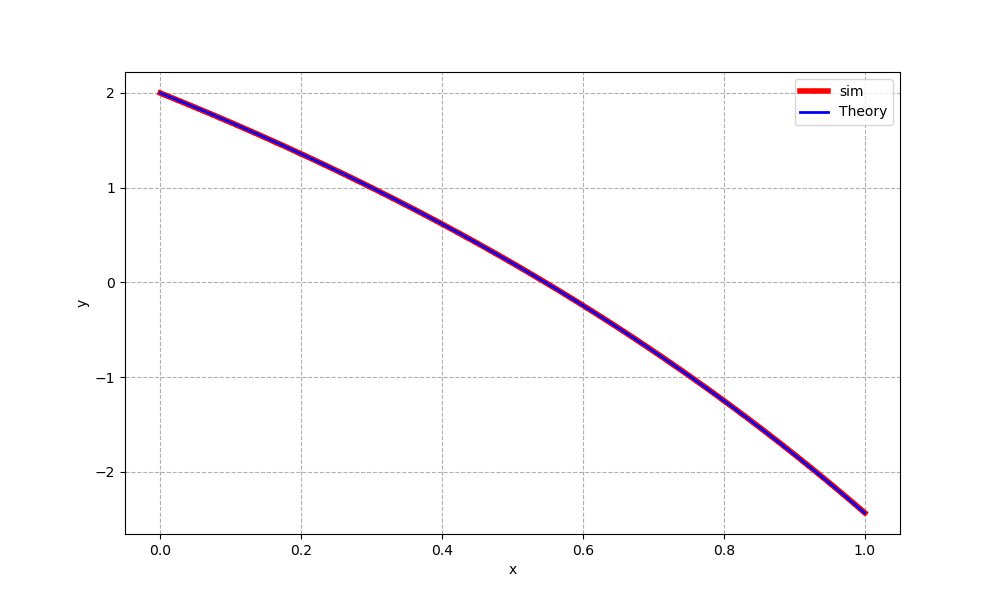
\includegraphics[width=\linewidth]{figs/Figure_1.png}
    \end{center}
\end{frame}




\end{document}
